% Chapter ApnaService

\chapter{APNA as SCION Service} % Main chapter title

\label{apna_service}

\section{APNA Service}
APNA Service (AP\_SVC) is radically different from the past two approaches described in previous chapters (Chap. \ref{apna_overlay}, \ref{address_family}). The main idea behind this approach is to create a new SCION service (like Path Service, Certificate Service) which would be responsible for forwarding APNA packets. The main advantage of this approach instead of modifying the border router and dispatcher to handle APNA packets this new service will take care of APNA packets instead. That makes this approach easily deployable on the current SCIONLab infrastructure without a lot of changes in the existing deployment.

APNA service is like a data plane service which is responsible for providing anonymous communication service for SCION. Any packet send to APNA service will get anonymously delivered to the destination. Source APNA service uses the anycast address to deliver the packet to destination APNA service which then forwards it to the appropriate host. Since we are using the anycast address for communication attacker cannot hamper the anonymity guarantees provided by APNA framework. 

\subsection{Communication Overview}
\begin{figure}[th!!]
\centering
\hspace*{-2cm}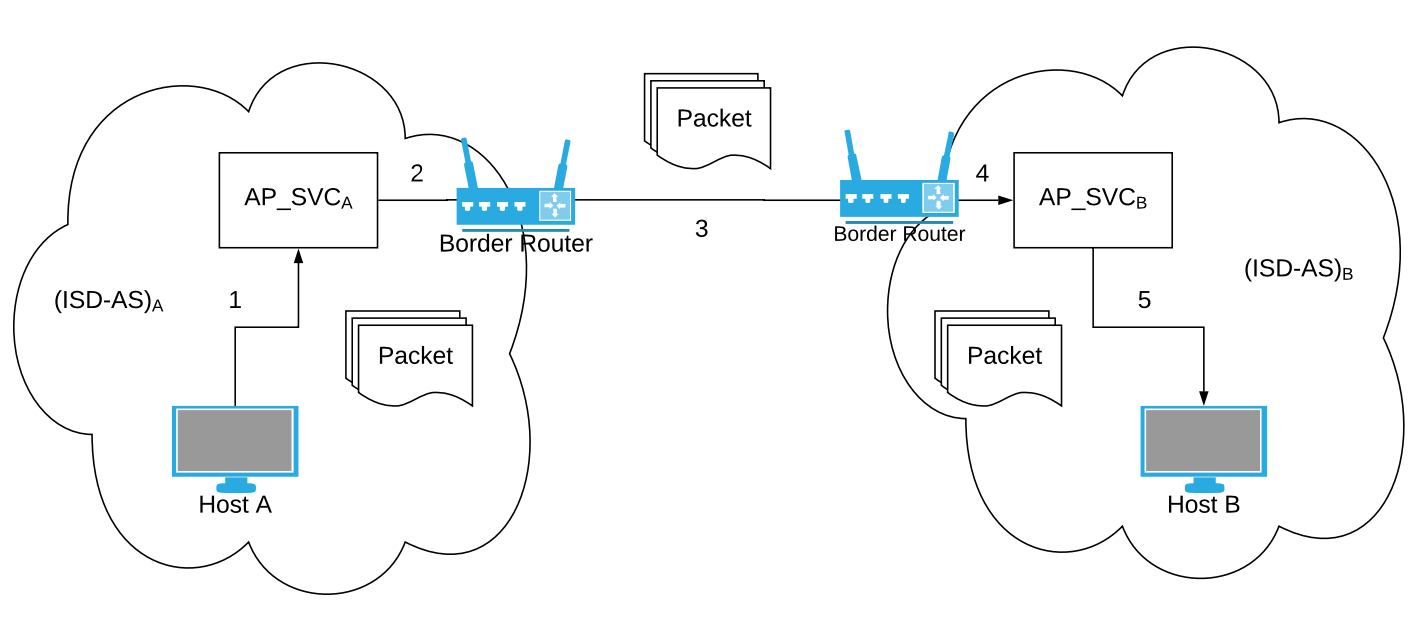
\includegraphics[scale=0.3]{Figures/svc_arch.png}
\decoRule
\caption[Communication overview for APNA Service]{Communication overview for APNA Service architecture}
\label{fig:srv_comm}
\end{figure}
In order to understand how does two parties communication using this new APNA Service. Let's take a simple scenario as presented in Fig.\ref{fig:srv_comm}. In this case Host A which is located in $(ISD-AS)_{A}$ wants to send a packet to Host B located in $(ISD-AS)_{B}$. Host A will forward the packet to APNA Service which is located in its AS and then it will verify the packet MAC. In the previous approach this MAC verification was handled Border Router. If its successful then it will forward that packet to another APNA Service located in the destination $(ISD-AS)_{B}$ using anycast address.

After receiving the packet APNA Service will verify if its a valid destination EphID. If its valid then it will decrypt the EphID to obtain the HostID to forward it to the appropriate host. Otherwise packet will be dropped.

\subsection{APNA Service Architecture}
APNA Service needs to be highly reliable and efficient and in order to achieve this goal, its designed as a highly concurrent service using go-routines. Each functionality of APNA Service is distributed among different go-routines in order to avoid bottlenecks and use the power of multiprocessing to the full extend. There are multiple go-channels and each channel has a go-routine associated with it and whenever a packet arrives it gets processed by the appropriate go-routine and forwarded to the next channel for further processing.

\subsection{Processing Outgoing Packet by APNA Service}
Firstly APNA Service reads the packet from the \textit{UDP} network socket and transfers that packet to the receive queue. Another go-routine will read packet from this receive queue and try to serialize the packet and if the serialization is successful it will be put into MAC Verification Queue. Otherwise it will be forwarded to error queue and a SCMP message will be sent to the sender of the packet.

If the packet reaches MAC verification queue another go-routine would perform MAC verification for the packet. If the packet has not been tampered then the MAC verification would succeed and forwarded to the forwarding queue. Otherwise packet would be dropped.

Forwarding queue go-routine would try to de-serialize the packet so that it could be forwarded to the border router which could deliver the packet to the destination. But if there is a error while de-serializing the packet and it would be moved to error queue and eventually a SCMP message will be sent to sender.
\begin{figure}[th!!]
\centering
\hspace*{-2cm}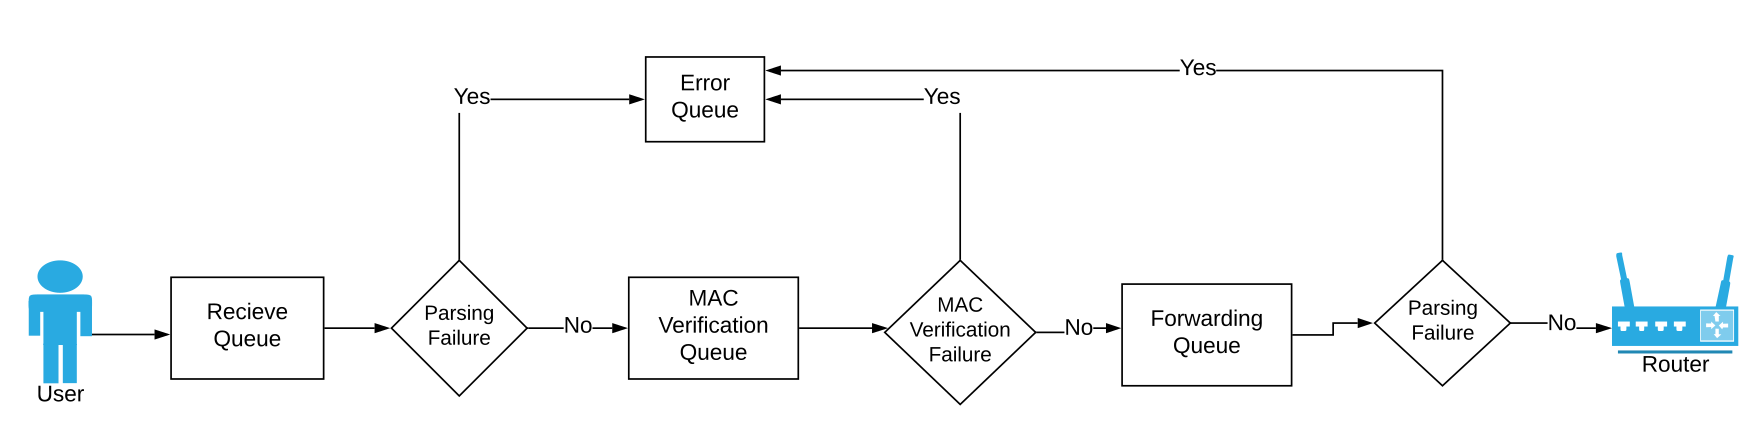
\includegraphics[scale=0.3]{Figures/svc.png}
\decoRule
\caption[APNA Service Outgoing Packet]{Outgoing Packet Processing by APNA Service}
\label{fig:perf_ephid}
\end{figure}

\subsection{Processing Incoming Packet by APNA Service}
\begin{figure}[th!!]
\centering
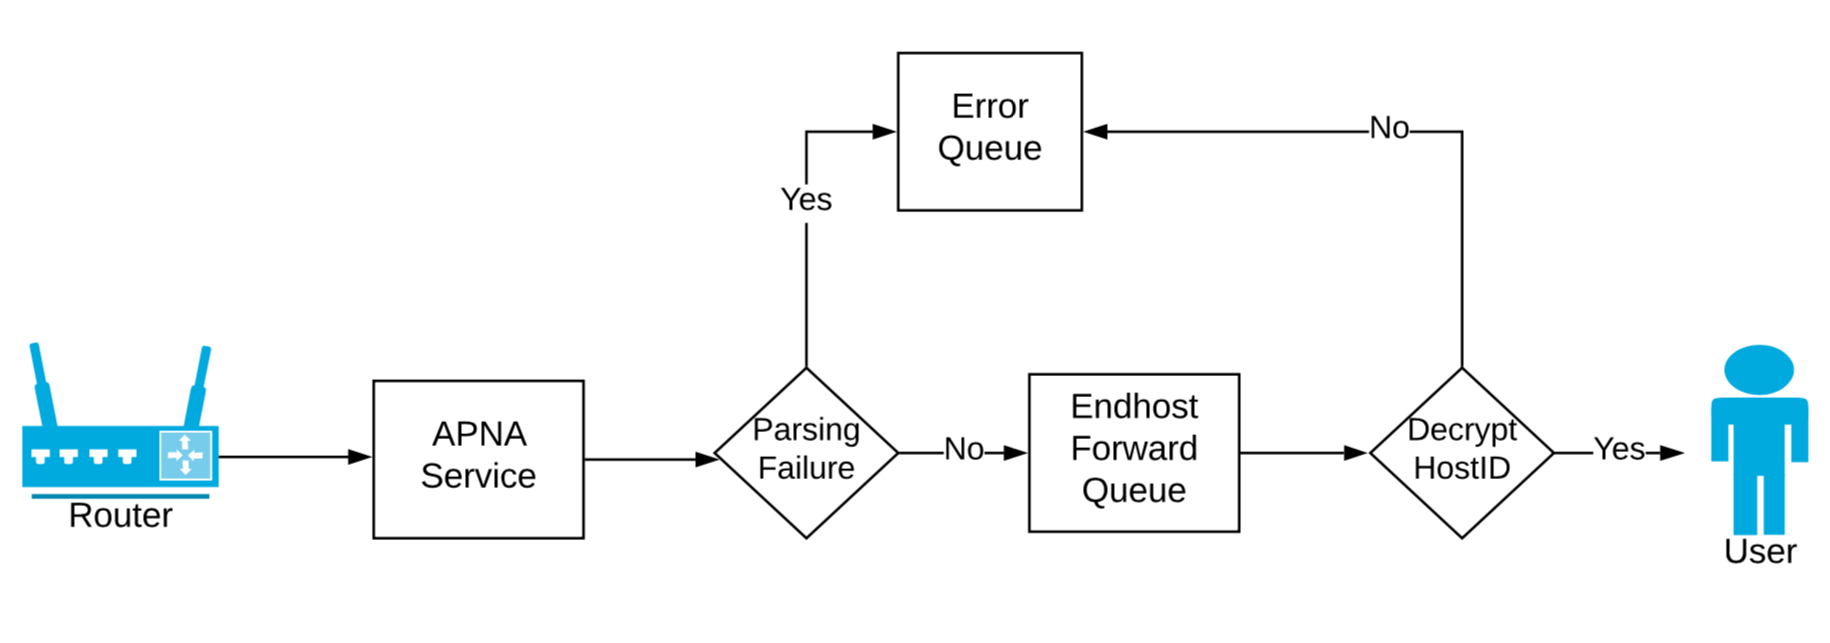
\includegraphics[scale=0.24]{Figures/svc_out.png}
\decoRule
\caption[APNA Service Incoming Packet]{Incoming Packet Processing by APNA Service}
\label{fig:perf_ephid}
\end{figure}

\section{Modifications in the current infrastructure}
\subsection{SNET}
There is a minor modification required in the existing snet implementation. First and foremost a new network string called "apna" needs to be introduced. Currently only one network is supported namely "udp4" but using this new network string we can modify the read and write functions to send/accept packets to/from APNA Service instead of directly forwarding it to border router or dispatcher.
\subsection{SCIOND}
SCIOND needs to be modified to resolve APNA Service Address (AP\_SVC)
\subsection{Border Router}
\subsection{SCION-APNA Packet Structure}
\begin{figure}[th!!]
\centering
\noindent
\makebox[\textwidth]{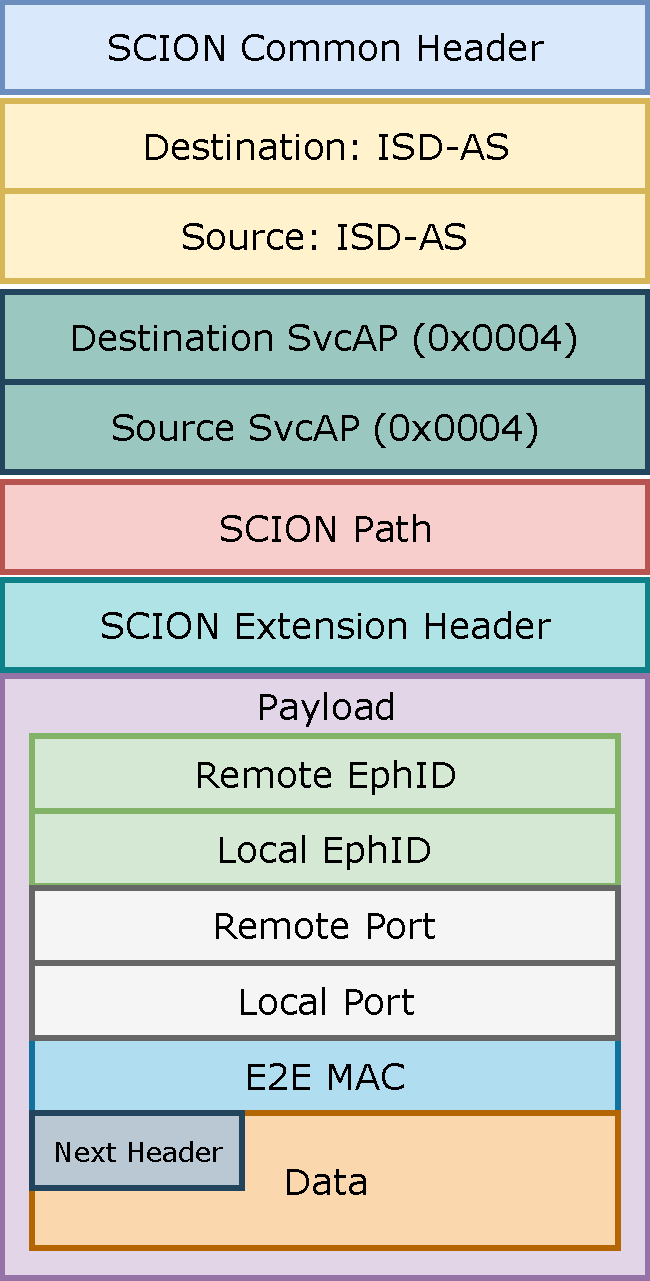
\includegraphics[scale=0.6]{Figures/apna_svc.pdf}}
\decoRule
\caption[APNA packet structure using SvcAP]{APNA packet structure  using SvcAP for forwarding APNA packets}
\end{figure}